\section{Reproducibility Summary}
\subsection{Scope of Reproducibility}
We replicate \citet{gao2021privacy}, which proposes an automatic search algorithm to find privacy-preserving transformation policies to protect against gradient reconstruction attacks in a collaborative learning setting. All the main claims made by the authors were tested. We also extend the original experiments to a new dataset, and contribute a PyTorch Lightning framework to aid in future work.

\subsection{Methodology}
We perform all experiments using the model architectures, hyperparameters and datasets as used in the original work. We also extend the experiments to a new dataset. We further contribute a reimplementation of the work in PyTorch Lightning to provide a modular framework for future research into this area. All experiments are performed on Nvidia GTX 1080 GPUs. Our logs and checkpoints are made available for download via our code repository.

\subsection{Results}
Overall we find the original results to be reproducible; transformation policies found using \citet{gao2021privacy}'s method can defend against gradient reconstruction attacks, and these transformations have negligible impact on training efficiency and model accuracy. However we do not observe the reported correlation between the proposed privacy-score $S_{pri}$ and reconstruction PSNR. We also find that the degree of protection differs greatly from image to image, with poor protection in the worst case.

\subsection{What was easy}

The original paper was clearly written and the general idea was easy to follow. There was a codebase available in PyTorch and some of the reported experiments were reproducible using this code.

\subsection{What was difficult}

The available codebase was not clearly structured and needed non-trivial work to run some of the experiments reported on in the paper. There were otherwise undocumented details in the code that had a large impact on experiment outcomes.

\subsection*{Communication with original authors}

\citet{gao2021privacy} were contacted about multiple issues regarding implementation details and notation clarifications. The authors were very receptive to our questions, and most of these were resolved swiftly and constructively.

\newpage

%%%%%%%%%%%%%%%%
% INTRODUCTION %
%%%%%%%%%%%%%%%%

\section{Introduction}
\label{sec:intro}

Collaborative learning systems enable multiple clients to jointly train a machine learning model. Each client locally holds a split of the training data, which they use to locally compute gradients \cite{yang2019federated}\cite{guo2020towards}\cite{melis2019exploiting}. These local gradients are then shared among all users to update the parameters of the shared model. This removes the need for any individual client to share potentially sensitive data, while still enabling all clients to benefit from a model trained on a larger dataset than they themselves own. This is an important quality in any field where data confidentiality is desired. As such, collaborative learning is used in applications from mobile networks \cite{kang2019} to autonomous driving \cite{niknam2020federated} and health care \cite{brisimi2018federated}.

However, it has been shown that training images may be recovered from the gradients that are shared to the network \cite{geiping2020inverting}\cite{zhao2020idlg}\cite{zhu2019}. In general, these \emph{reconstruction attacks} mask as harmless peers to obtain a shared model state and gradient from the victim, initialize a random input image and subsequently optimize this input such that the model gradient closely matches the victim's gradient. The end result is an approximation of the victim's input image, breaking confidentiality and invalidating the core principles of this style of collaborative learning.

\citet{gao2021privacy} propose a novel approach to mitigate the threat from reconstruction attacks by augmenting the local training data of the user before calculating the gradients \cite{gao2021privacy}. The augmentation is aimed at making the reconstruction attack prohibitively difficult. The authors develop an automatic search algorithm to find the optimal transformation policies to augment the data and propose two novel metrics, $S_{pri}$ and $S_{acc}$, to increase the efficiency of this search.

In this reproducibility report, we evaluate the main claims made by the authors of \cite{gao2021privacy} by reproducing their techinques and experiments. Moreover, we assess the availability of hyperparameters and other information needed for reproducibility, and we discuss the usability of the provided codebase. We also extend the experimental setup towards a new dataset and contribute a new, PyTorch Lightning-based framework to enable future work.

%%%%%%%%%%%%%%%%%%%%%%%%%%%%
% SCOPE OF REPRODUCABILITY %
%%%%%%%%%%%%%%%%%%%%%%%%%%%%

\section{Scope of reproducibility}
\label{sec:claims}

The original paper \cite{gao2021privacy} proposes using data augmentation to make gradient reconstruction attacks in a collaborative learning setting prohibitively difficult. To find transformation policies that achieve this goal, an automatic search algorithm is developed. Additionally, to make the proposed algorithm computationally feasible, the authors devise two novel metrics described in Section \ref{sec:3.2search}. We split these contributions into the following 7 claims and refer to them throughout this report.

\begin{itemize}[noitemsep]
\item \textbf{Claim 1}: By  augmenting training samples with carefully-selected transformation  policies,  reconstruction attacks become infeasible.
\item \textbf{Claim 2}: The proposed search algorithm can find effective and general policies -- policies that are able to defeat multiple variants of reconstruction attacks.
\item \textbf{Claim 3}: The found policies are highly transferable; good policies searched for one dataset are also suitable for another.
\item \textbf{Claim 4}: The found policies have negligible impact on training efficiency.
\item \textbf{Claim 5}: In general, a good policy is made up of transformations that distort the details of the training samples, while maintaining the semantic information.
\item \textbf{Claim 6}: The five transformations that work best are \emph{horizontal shifting (9)}, \emph{brightness (9)}, \emph{brightness (6)}, \emph{contrast (7)} and \emph{contrast (6)}. Here, the number inside the brackets represents the intensity of the applied transformation.
\item \textbf{Claim 7}: $S_{pri}$ is a good measure of privacy; it is linearly correlated to Peak Signal-to-Noise Ratio (PSNR) \cite{hore2010} with a Pearson Coefficient \cite{stigler1989} of $0.697$.
\end{itemize}

In \cite{gao2021privacy}, each of these claims is accompanied by one or more experiments, the results of which are reported in various tables and figures. In this reproducibility study we rerun the experiments and reproduce their tables and figures, with the addition that we report standard deviations across several experiments. In Section \ref{sec:results}, we present our results side-by-side with the original work. Then, in Section \ref{sec:discussion}, we discuss the reproducibility of each experiment and evaluate the validity of the claims.\bigskip

In addition to testing the above claims from the original paper, we present two extensions. Both of these extensions are aimed at testing the transferability of the searched policies as claimed in \emph{Claim 3}.

\begin{itemize}[noitemsep]
    \item \textbf{Extension 1}: Using the policies searched on one dataset and applying them to a new dataset can make reconstruction attacks against this new dataset infeasible
    \item \textbf{Extension 2}: Since good policies share the same general qualities, as claimed by \emph{Claim 5}, the five best transformations from \emph{Claim 6} are the same when using a different dataset.
\end{itemize}

Again, we show the results for these extension in Section \ref{sec:results}, and relate them to the original claims, experiments and results in Section \ref{sec:discussion}.

%%%%%%%%%%%%%%%%%%%%%%%%%%%%%%%%%%%%%%%%%%%%%%%%%%%%%%
% FINDING PRIVACY-PRESERVING TRANSFORMATION POLICIES %
%%%%%%%%%%%%%%%%%%%%%%%%%%%%%%%%%%%%%%%%%%%%%%%%%%%%%%

\section{Finding privacy-preserving transformation policies}

The original paper proposes an automatic search algorithm for finding privacy-preserving transformation policies. To better understand this contribution, we describe what constitutes a transformation policy and how good policies are found within a reasonable time.

\subsection{Transformation policies}

Transformations or augmentations have been widely used to improve model performance and generalizability in deep learning. In \cite{gao2021privacy}, transformations from AutoAugment \cite{cubuk2019autoaugment} are repurposed to protect sensitive training data from reconstruction attacks. The library contains $50$ different transformations, including rotation, crop, shift, inversion, brightness, and contrast. A \emph{transformation policy} is a combination of $k$ such transformations applied sequentially to each of the training samples. In \cite{gao2021privacy}, $k=3$ is chosen and the policies are denoted by the indices of the transformations within the AutoAugment library.

It should be noted that while augmented samples are usually \emph{added} to the training set, here the augmented version \emph{replace} the originals. Therefore consistently applying the best policy to the data would risk a distribution shift in the dataset. Therefore, the authors propose the \emph{hybrid strategy}, where a random policy from $3$ candidate policies is used in order to preserve the input distribution \cite{gao2021privacy}.

\subsection{Reducing the search space}
\label{sec:3.2search}

To find candidate policies, it is necessary to determine their effect on both privacy and accuracy. The transformations must be applied to training data, and a model must be trained. Because fully training a model is computationally expensive, the authors propose two metrics that serve as a proxy for the privacy preservation and accuracy of the fully trained model: a privacy score ($S_{pri}$) and an accuracy score ($S_{acc}$). Low $S_{pri}$ means the model has high privacy preservation potential, and high $S_{acc}$ means the model achieves good accuracy with the applied transformation policies. These metrics produce results on model that are trained with only $10\%$ of the data for only $25\%$ training iterations, reducing the search space and making the policy search feasible in a reasonable time. Further details about the definition of $S_{pri}$ and $S_{acc}$ can be found in sections $4.2$ and $4.3$ of \cite{gao2021privacy}.

\section{Experimental setup and code}

To verify the claims made by the authors of \cite{gao2021privacy}, we reproduce their experiments. These experiments roughly fall into four categories: evaluating the effectiveness of the searched policies against reconstruction attacks, testing the transferability of the searched policies on different datasets and models, checking the impact on model efficiency, and studying the semantics behind the different transformations. Multiple models must be trained on augmented and un-augmented data for all these categories. For the attacks, the approach from \cite{geiping2020inverting} is applied. Section \ref{sec:results} provides a detailed description of the experiments and shows the results.

To reproduce the experiments performed by the authors, we used their existing codebase\footnote{\url{https://github.com/gaow0007/ATSPrivacy}}, which is implemented in PyTorch \cite{pytorch2019}. We reimplemented the code in PyTorch Lightning\footnote{\url{https://github.com/PyTorchLightning/pytorch-lightning}}, which leverages the interface advantages of the Lightning framework to make running experiments, logging results and extending the work more intuitive. It is publicly available at \url{github.com/stfwn/ats-privacy-replication}.

\subsection{Datasets}

The experiments in \cite{gao2021privacy} are performed on two datasets, CIFAR-100\footnote{\url{https://www.cs.toronto.edu/~kriz/cifar.html}} \cite{krizhevsky2009learning}, and Fashion-MNIST\footnote{\url{https://github.com/zalandoresearch/fashion-mnist}} \cite{xiao2017fashionmnist}. CIFAR-100 contains $60,000$ color images of size $32\times32$, from $100$ classes. The test set is used as the validation set, consistent with the authors' codebase.
On the other hand, the Fashion-MNIST dataset contains $70,000$  grey-scale images of $28\times28$ resolution from $10$ classes. Again the test set is used as a validation set. We run experiments on one additional dataset in our extensions - Tiny ImageNet200\footnote{\url{http://cs231n.stanford.edu/tiny-imagenet-200.zip}} \cite{imagenet_cvpr09}. It contains 120,000, $64\times64$ RGB images of 200 different classes. However, a \emph{tiny} version of the dataset is introduced in the original paper for policy-search purposes. This dataset version contains $10\%$ of the original samples, using the same distribution. It's later used to train the models for the evaluation of $S_{pri}$ and $S_{acc}$ in the search algorithm.

\subsection{Model descriptions}

We use the following models:

\begin{itemize}[noitemsep]
    \item ResNet20-4, a variation of ResNet20~\cite{he2016deep} that has four times the number of channels also used in \cite{geiping2020inverting}. The total number of parameters is 4.4M.
    \item ConvNet~\cite{geiping2020inverting} -- an 8-layer Convolutional Neural Network, with batch normalization and a ReLU layer after each convolution layer. For this model the total number of parameters is 3.7M.
\end{itemize}

The original codebase uses the implementation of both models from the repository\footnote{https://github.com/JonasGeiping/invertinggradients} of \cite{geiping2020inverting}. Our models are exact reimplemations in Pytorch Lightning.

\subsection{Hyperparameters}

For the policy search, we set $C_{max} = 1500$ and \emph{max policies} equal to 10. The batch size was $128$, and the number of transforms in policy was $3$.

For training, the batch size was also $128$ and the number of epochs was $60$ (see Section \ref{section:computational-requirements}). To obtain a semi-trained network, we used a subset of $10\%$ of the training dataset. Attacks are performed on the first six images of the test set, and we used the configurations as described in the original paper. An exception is the experiment that led to Figure \ref{fig:2}, where the original configuration was unclear.

\subsection{Computational requirements}
\label{section:computational-requirements}

We ran our experiments using an Nvidia GeForce GTX 1080 GPU. The policy search took approximately $10$ hours. The training of one model took approximately 2h 40min using the original approach. However, training for $60$ epochs achieves the same accuracy in only $50$ minutes by reducing the learning rate sooner, thereby skipping long periods of stagnation. Performing one reconstruction attack in $2500$ iterations took approximately $5$ minutes. Measuring the correlation between $S_{pri}$ and PSNR therefore took $8.5$ hours (including policy search).

%%%%%%%%%%%%%%%%%%%%%%%%%%%
% EXPERIMENTS AND RESULTS %
%%%%%%%%%%%%%%%%%%%%%%%%%%%

\section{Experiments and results}
\label{sec:results}

\subsection{Results reproducing original paper}

\paragraph{Experiment 1} A reconstruction attack on $100$ images from the CIFAR-100 validation set is performed with and without a searched transformation policy applied. We document the optimization process of the attack in terms of GradSim. The model used is ResNet20, trained on the tiny dataset for $50$ epochs. The results of this experiment are shown in Figure \ref{fig:1re}, which shows a very similar result to the original paper shown in \ref{fig:1og}. In addition to the original figure, we show the standard deviation over the $100$ images, since GradSim can differ significantly from image to image. When taking the average of multiple runs, it can be seen that the privacy-aware transform does indeed make the GradSim convergence more difficult.
\setcounter{figure}{-1}    
\begin{figure}[h]
        \centering
        \subfloat[Reproduced result]{
            \includegraphics[width=0.4\textwidth]{images/fig1.png}
            \label{fig:1re}
        }
        \subfloat[Original result]{
            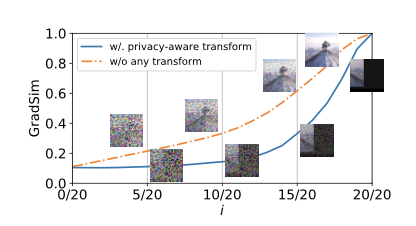
\includegraphics[width=0.4\textwidth]{images/fig1OG.png}
            \label{fig:1og}
        }
        \captionof{figure}{Optimization process of reconstruction attack with and without searched policy}
        \label{fig:1}
\end{figure}
\setcounter{figure}{0} 
\begin{figure}[h]
        \centering
        \subfloat[Reproduced result]{
            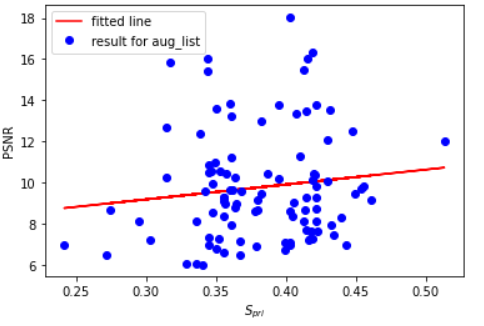
\includegraphics[width=0.4\textwidth]{images/fig2.png}
            \label{fig:2re}
        }
        \hspace{5mm}
        \subfloat[Original result]{
            \includegraphics[width=0.4\textwidth]{images/fig2og.png}
            \label{fig:2og}
        }
        \captionof{figure}{Correlation between $S_{pri}$ and PSNR}
        \label{fig:2}
    \vspace{-5mm}
\end{figure}

\paragraph{Experiment 2} A visual comparison between reconstructed images with and without a searched transformation policy applied is performed for both ResNet20 and ConvNet on images from CIFAR-100 and Fashion-MNIST. The optimizer used in the attack is Adam+Cosine. The images, the resulting reconstructions, and their PSNR values are shown in the left half of Figure \ref{fig:4}. The results from the original paper are shown at the right side of Figure \ref{fig:4}. As can be seen, the images used and PSNR values reported are different. This is due to the fact that it was too expensive to identify the exact same images and PSNR values differ quite severely depending on the image used. However, for all $12$ images, we observe a less pronounced visual effect of the transformation policy as well as a smaller gap in PSNR values between the reconstructions with and without the policies applied. This implicates that the effect shown in the original paper is not as severe for all images, although the images we selected may be particularly easy to reconstruct.

\begin{figure}[h]
\centering
    \subfloat[CIFAR-100 with ResNet20]{
        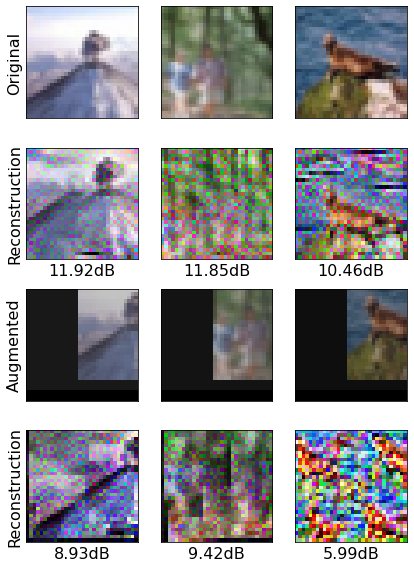
\includegraphics[width=0.24\textwidth]{images/fig4a.png}
        \label{fig:4a}
    }
    \subfloat[CIFAR-100 with ConvNet]{
        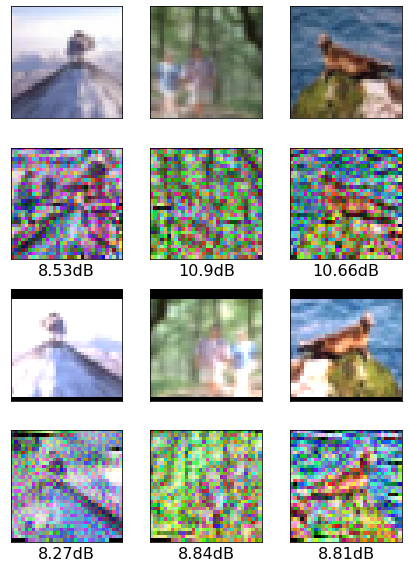
\includegraphics[width=0.24\textwidth]{images/fig4b.png}
        \label{fig:4b}
    }
    \subfloat[FMNIST with ResNet20]{
        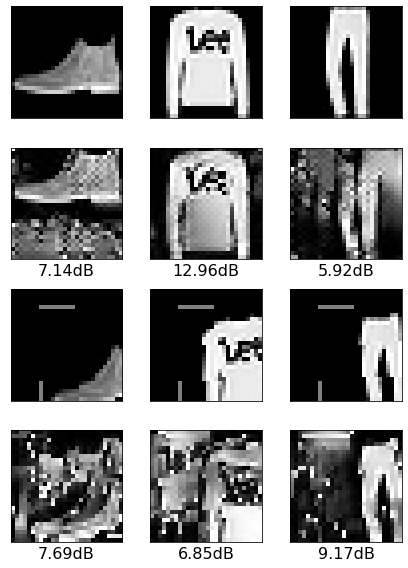
\includegraphics[width=0.23\textwidth]{images/fig4c.png}
        \label{fig:4c}
    }
    \subfloat[FMNIST with ConvNet]{
        \includegraphics[width=0.23\textwidth]{images/fig4d.png}
        \label{fig:4d}
    }
    
    \subfloat[CIFAR-100 with ResNet20]{
        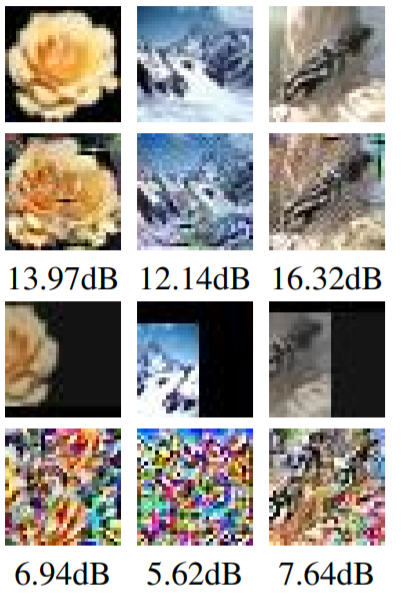
\includegraphics[width=0.24\textwidth]{images/fig4aog.PNG}
        \label{fig:4aog}
    }
    \subfloat[CIFAR-100 with ConvNet]{
        \includegraphics[width=0.24\textwidth]{images/fig4bog.PNG}
        \label{fig:4bog}
    }
    \subfloat[FMNIST with ResNet20]{
        \includegraphics[width=0.23\textwidth]{images/fig4cog.PNG}
        \label{fig:4cog}
    }
    \subfloat[FMNIST with ConvNet]{
        \includegraphics[width=0.23\textwidth]{images/fig4dog.PNG}
        \label{fig:4dog}
    }
    \caption{Visualization results for reconstruction attacks on different datasets and models with associated PSNR values. Our results above and original results below.}
    \label{fig:4}
\end{figure}

\paragraph{Experiment 3}

To gain further insight into the effectiveness of the different policies, we report the qualitative and quantitative results of Adam+Cosine attacks and model accuracy for the datasets and models in Figure \ref{fig:4}. The results are calculated over $6$ images as performing the experiment is very expensive and number wasn't stated in the paper. The policies considered and the results are listed in Table \ref{tab:1}.
\begin{center}
\begin{table}[h]
    \begin{subtable}[h]{0.25\textwidth}
      \begin{tabular}{lrrr}
            \hline
             Policy   &   PSNR &   PSNR (std) &   Acc \\
            \hline
             None     &       12.15 &       2.06 & 78.11 \\
             Random   &        9.92 &       1.93 & 75.02 \\
             3-1-7    &        6.77 &       0.88 & 71.59 \\
             43-18-18 &        9.34 &       1.81 & 77.16 \\
             Hybrid   &        8.25 &       1.64 & 77.47 \\
            \hline
        \end{tabular}
        \caption{CIFAR-100 + ResNet20}
    \end{subtable}
    \hspace{40mm}% \hfill
    \begin{subtable}[h]{0.25\textwidth}
        \begin{tabular}{lrrr}
            \hline
             Policy   &   PSNR &   PSNR (std) &   Acc \\
            \hline
             None     &       11.44 &       2.93 & 72.97 \\
             Random   &       10.29 &       1.02 & 71.93 \\
             21-13-3  &        8.23 &       2.18 & 63.26 \\
             7-4-15   &       10.31 &       2.14 & 70.77 \\
             Hybrid   &        9.89 &       1.47 & 68.91 \\
            \hline
        \end{tabular}
        \caption{CIFAR-100 + ConvNet}
    \end{subtable}
    \vfill
    \vspace{0mm}
    \begin{subtable}[h]{0.25\textwidth}
        \begin{tabular}{lrrr}
            \hline
             Policy   &   PSNR &   PSNR (std) &   Acc \\
            \hline
             None     &        9.81 &       4.41 & 95.19 \\
             Random   &       10.06 &       2.04 & 95.19 \\
             19-15-45 &        8.26 &       0.37 & 92.44 \\
             2-43-21  &        8.93 &       2.93 & 93.93 \\
             Hybrid   &        8.41 &       1.45 & 95.14 \\
            \hline
        \end{tabular}
        \caption{FMINST + ResNet20}
    \end{subtable}
    \hspace{40mm}% \hfill
    \begin{subtable}[h]{0.25\textwidth}
        \begin{tabular}{lrrr}
            \hline
             Policy   &   PSNR &   PSNR (std) &   Acc \\
            \hline
             None     &        9.52 &       3.27 & 94.61 \\
             Random   &        9.47 &       2.27 & 94.47 \\
             42-28-42 &        7.59 &       0.89 & 94.62 \\
             14-48-48 &        8.41 &       2.10 & 94.68 \\
             Hybrid   &        6.80 &       0.98 & 94.59 \\
            \hline
        \end{tabular}
        \caption{FMNIST + ConvNet}
    \end{subtable}
    \caption{PSNR (db) (including mean and standard deviation over $6$ images) and model accuracy (\%) of different transformation configurations for each model and dataset. $19-1-18$ is the random policy.}
    \label{tab:1}
\end{table}
\end{center}
Table \ref{tab:1} shows similar patterns to the original paper, where the searched policies have low PSNR values compared to not using transformations. We do observe that PSNR values have a relatively high standard deviation, and during our experiments, we found that the policies do not form a good defense for some images. This problem will be further discussed in Section \ref{sec:discussion}.

\paragraph{Experiment 4} The defensive qualities of the searched transformation policies are benchmarked against existing defenses from the literature \cite{zhu2019} \cite{wei2020} under the Adam+Cosine attack. The results are shown in Table \ref{tab:3}. Although the exact values differ slightly, the overall results are similar to the original paper, where all the existing defenses perform worse than the hybrid strategy.

\paragraph{Experiment 5} This experiment concerns \textbf{Claim 2}. Because policies should be general, they are tested against various attack configurations. For this, we again use $6$ images from the test set and perform the different attacks on the images without the transformation policies applied and with the hybrid strategy transformation policies applied. The results are shown in Table \ref{tab:2}. As can be seen from the table, the hybrid strategy works well against all configurations of the reconstruction attack. This is in line with the results from the original paper.

\begin{table}[htb!]
    \centering
    \begin{tabular}{lrrrr}
        \hline
         Attack       &   None &   None  (std) &   Hybrid &   Hybrid  (std) \\
        \hline
         LBFGS+L2     &               8.61 &             1.22 &                 6.33 &                2.00 \\
         Adam+Cosine  &              12.15 &             2.06 &                 8.25 &                1.64 \\
         LBFGS+Cosine &               9.62 &             0.91 &                 7.47 &                0.25 \\
         Adam+L1      &               9.48 &             0.71 &                 6.43 &                0.16 \\
         Adam+L2      &               9.28 &             0.69 &                 6.46 &                0.21 \\
         SGD+Cosine   &              12.60 &             2.07 &                 8.03 &                1.47 \\
        \hline
        \end{tabular}
    \caption{PSNR values (db) (including mean and standard deviation over $6$ images) of reconstructed images with and without transformations applied for different attack configurations}
    \label{tab:2}
\end{table}
\begin{table}[htb!]
    \centering
        \begin{tabular}{lrr}
            \hline
             Policy   &   PSNR &   PSNR std \\
            \hline
             None     &       15.39 &       2.78 \\
             3-1-7    &        8.47 &       0.85 \\
             43-18-18 &       10.97 &       1.06 \\
             Hybrid   &        8.95 &       0.90 \\
            \hline
        \end{tabular}
    \caption{CIFAR100 with ResNet20}
    \label{tab:my_label}
\end{table}

\paragraph{Experiment 6} This experiment concerns the transferability of \textbf{Claim 3}. To test this, the policies searched on CIFAR-100 are applied to Fashion-MNIST using both ResNet20 and ConvNet. Reconstruction attacks are performed with the Adam+Cosine attack. The resulting PSNR values and accuracies are listed in Table \ref{tab:4}. The results differ from the original. It can be seen that the transformation policies are not effective here.

\begin{table}[h]
    \centering
    \begin{subtable}[h]{0.4\textwidth}
    \centering
        \begin{tabular}{lrrr}
            \hline
             Policy   &   PSNR &   PSNR (std) &   Acc \\
            \hline
             None     &        9.81 &       4.41 & 95.19 \\
             3-1-7    &        9.30 &       2.72 & 93.20 \\
             43-18-18 &       10.03 &       2.23 & 94.88 \\
             Hybrid   &        7.49 &       1.57 & 94.49 \\
            \hline
        \end{tabular}
        \caption{FMNIST + ResNet20}
    \end{subtable}
    \hspace{10mm}
    \begin{subtable}[h]{0.4\textwidth}
    \centering
        \begin{tabular}{lrrr}
            \hline
             Policy   &   PSNR &   PSNR (std) &   Acc \\
            \hline
             None     &        9.52 &       3.27 & 94.61 \\
             21-13-3  &        9.99 &       2.12 & 92.38 \\
             7-4-15   &        9.34 &       1.62 & 94.35 \\
             Hybrid   &       11.50 &       5.80 & 93.77 \\
            \hline
        \end{tabular}
        \caption{FMNIST + ConvNet}
    \end{subtable}
    \caption{Resulting PSNR (dB) and accuracy (\%) values for applying policies searched on CIFAR-100 to Fashion-MINST}
    \label{tab:4}
\end{table}

\paragraph{Experiment 7}

The following experiment is aimed at \textbf{Claim 4}. The authors state that applying the search policies has a negligible impact on training efficiency. We trained ResNet20 with the searched policies applied and documented the loss and accuracy convergence to test this. From Figure \ref{fig:3} it can be seen that indeed applying transformations has almost zero impact on the training efficiency. It is also noteworthy to observe that the training curves are almost identical compared with the results from the original work.

\begin{figure}[h]
    \centering
    \subfloat[Reproduced result]{
        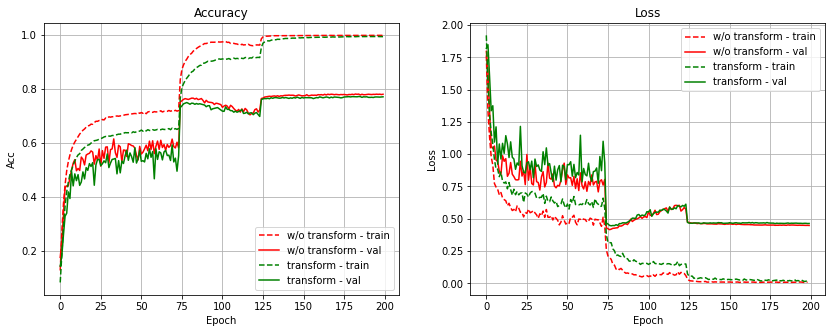
\includegraphics[width=0.5\textwidth]{images/fig3.png}
        \label{fig:3a}
    }
    
    \subfloat[Original result]{
        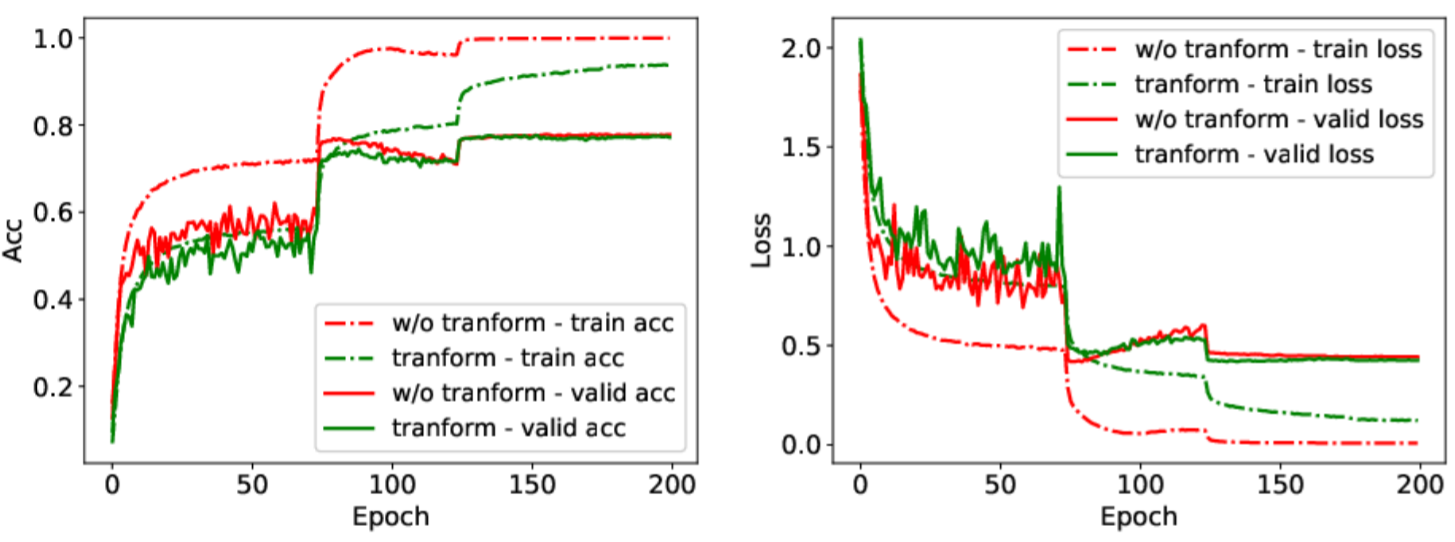
\includegraphics[width=0.5\textwidth]{images/fig3og.png}
        \label{fig:3b}
    }
    \caption{Convergence speed with and without transformations applied}
    \label{fig:3}
\end{figure}
\paragraph{Experiment 8}

\textbf{Claim 5} states that good transformation policies obfuscate details in the training samples but maintain high-order semantic information. As such, attackers will have trouble reconstructing high frequency information. We test this by comparing the attacker-defender gradient similarity during an attack of models trained with the searched policy, a random policy, and no policy applied. From Figure \ref{fig:6}, it can be seen that in shallow layers, the gradients differ significantly, whereas in deep layers, the gradients are very similar. This implies that the transformations do indeed have the desired effect and is in line with the results from the original paper.

\begin{figure}[htb]
    \centering
    \subfloat[Shallow layers]{
        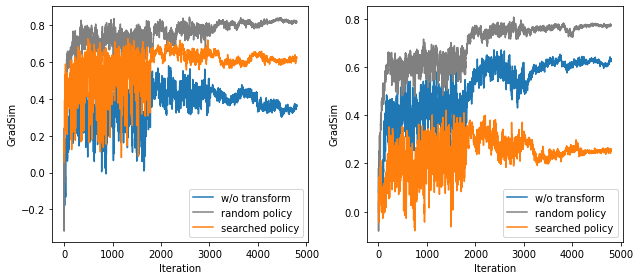
\includegraphics[width=0.5\textwidth]{images/fig6shallow.png}
        \label{fig:6a}
    }
    
    \hspace{5mm}
    \subfloat[Deep layers]{
        \includegraphics[width=0.5\textwidth]{images/fig6deep.png}
        \label{fig:6b}
    }
    \caption{Reproduced result of gradient similarity during the reconstruction optimization, for CIFAR100 with ResNet20}
    \label{fig:6}
    \vspace{-5mm}
\end{figure}

\paragraph{Experiment 9} In \textbf{Claim 6} the authors report their $5$ top transformations. We test whether we can find the same ones by calculating the privacy score on the dataset for each individual augmentation and show the results in Figure \ref{fig:5re} and \ref{fig:5og}. Out of the best $5$ transformations reported in the original paper we found $4$ overlapping ones. 

\begin{figure}[h]
    \centering
    \subfloat[Reproduced result]{
        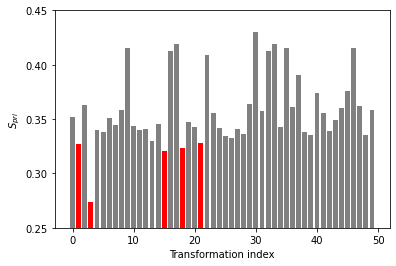
\includegraphics[width=0.3\textwidth]{images/fig5.png}
        \label{fig:5re}
    }
    \hspace{5mm}
    \subfloat[Original results]{
        \includegraphics[width=0.3\textwidth]{images/fig5og.png}
        \label{fig:5og}
    }
    \subfloat[Results on Tiny ImageNet]{
        \includegraphics[width=0.3\textwidth]{images/figext1.png}
        \label{fig:ext1}
    }
    \caption{Privacy scores of the 50 transformation functions in the augmentation library, best transformations are red.}
    \label{fig:5}
\end{figure}

\paragraph{Experiment 10}

The final experiment reproducing the results from the original paper is aimed at \textbf{Claim 7}. The authors claim that their privacy-score $S_{pri}$ is linearly correlated with PSNR with a Pearson-coefficient of $0.697$. We test this by running attacks and evaluating $S_{pri}$ on the model trained on tiny cifar100 for 50 epochs and found a very different result. As shown in Figure \ref{fig:2} there is hardly any correlation (Pearson-coefficient is $0.123$). This might be due to the fact that these $100$ transformation policies are selected at random out of $127.550$ possible options. This is a striking result nonetheless, which we discuss in-depth in Section \ref{sec:discussion}.

\subsection{Results beyond original paper}

\paragraph{Extension 1} We extend the evaluation of the transferability of the searched policies by evaluating the performance of the policy searched on CIFAR-100 on Rescaled ImageNet. The resulting PSNR values and accuracies are shown in Table \ref{tab:ext1}. As can be seen from the table, the hybrid strategy produces only $1$ dB improvement in PSNR value, and accuracy decreases by more than $4\%$. This weakens the claim of transferability made by the authors.

\paragraph{Extension 2} We additionally extend the evaluation of the transferability of the searched policies by testing which transformations work best on a different dataset. Since good policies share the same general qualities, as stated in Claim 5, the five best transformations from Claim 6 can be expected to be the same when using a different dataset. For this experiment, we use the Rescaled ImageNet dataset. The resulting transformations are shown in Figure \ref{fig:ext1}. Out of the $5$ best transformations on the Rescaled ImageNet $3$ were also found on CIFAR-100 in both our results and the results from the original paper. This shows that, indeed, these transformations contain the desired qualities from Claim 6.

\begin{table}[htb]
    \centering
    \begin{tabular}{lrrr}
        \hline
         Policy   &   PSNR &   PSNR (std) &   Acc \\
        \hline
         None     &        8.96 &       1.25 & 61.44 \\
         Hybrid   &        7.92 &       0.79 & 57.38 \\
        \hline
    \end{tabular}
    \caption{PSNR values (dB) and accuracies of policies searched on CIFAR-100 applied to Rescaled ImageNet}
    \label{tab:ext1}
\end{table}
\begin{table}[htb]
    \centering
        \begin{tabular}{lrrr}
        \hline
         Defense               &   PSNR &   PSNR (std) &   Acc \\
        \hline
         Pruning (70\%)         &       11.62 &       2.18 & 74.61 \\
         Pruning (95\%)         &       10.41 &       1.32 & 67.91 \\
         Pruning (99\%)         &        9.96 &       0.57 & 53.43 \\
         Laplacian ($10^{-3}$) &       10.73 &       1.02 & 71.45 \\
         Laplacian ($10^{-2}$) &       12.03 &       0.79 & 26.20 \\
         Gaussian ($10^{-3}$)  &       12.11 &       2.98 & 72.89 \\
         Gaussian ($10^{-2}$)  &       12.13 &       1.14 & 36.25 \\
        \hline
    \end{tabular}
    \caption{Comparisons with existing defense methods under the Adam+Cosine attack}
    \label{tab:3}
    \vspace{-8mm}
\end{table}

\section{Discussion}
\label{sec:discussion}

Overall the results in \cite{gao2021privacy} are reproducible, except Figure \ref{fig:2}, with a large discrepancy between our result and the original one -  we are still in contact with the authors on this issue. Nevertheless, augmentation policies tend to work as a defense mechanism rather well. For most images, an attacker using reconstruction attacks is unable to find privacy-sensitive information. However, the standard deviation of our results is more than $25\%$ in some settings, and we consider this a valuable metric to contribute. Some images are vulnerable to the attack even with the proposed defense mechanism, and it is as of yet unclear to us which types of images are more vulnerable than others. This issue must be developed further in future research to make the approach widely applicable in real-world use-cases where private data is at stake.

Additionally, we made observations in the codebase that, to the best of our knowledge, were not reported in the paper or any other accompanying documentation. The first was the fact that the loss of the training module was multiplied by a factor of $0.5$. This is not a fundamental flaw during the training phase, as it simply produces smaller gradients and therefore leads to a reduced effective learning rate. However, during the reconstruction attacks, the loss used by the attacker was not multiplied by this factor. This makes the attacker in practice use a different loss function from the one used to generate the gradient that it is attempting to match. This may therefore make reconstruction more difficult. Furthermore, we found that two other undocumented augmentations were added in all experiments, namely a random crop and random horizontal flip. Without these, the accuracy of our models decreased by over $10\%$. We are in contact with the authors regarding these observations, they acknowledged the halved loss as a bug.

\subsection{What was easy}

The explanation of the general idea and solution of the paper was very clearly put and easy to follow. The codebase contained a README with instructions on how to run some of the paper's experiments, and these instructions could be followed without significant problems. The code produced results as seen in the paper.

\subsection{What was difficult}

The most challenging part about reproduction was the unclear description of experiments in the paper and limited clarity in the codebase. Code in the repository was uncommented, used many global variables and many layers of indirection. Many chunks of code were not used, making it harder to follow. Some experimental settings and metrics were not implemented, and some experiment configurations led to fatal errors.

It was very unclear which steps were originally followed to obtain Figure \ref{fig:2}. Despite the authors' helpful comment on which model was used, we were not able to reproduce the correlation, potentially due to randomness in a vast search space (127,550) and the limited sample size (100). Furthermore, the paper does not state how many images were used to produce the PSNR values in the tables. Finally, undocumented augmentations were added in some but not all settings, which was cause for some delay until this was found to be the cause for a 10\% accuracy-gap with the authors' results.

\subsection{Communication with original authors}

We contacted the authors about multiple clarifications regarding implementation details and notation in the paper. The authors responded promptly and answered almost all of our questions in the first round of contact. We are still in contact on two points. Firstly, regarding our reproduction of Figure \ref{fig:2}. Since we got such differing results for this critical part of the authors' work, we are looking to investigate this further and possibly resolve the discrepancy with them. Secondly, we offered our refactoring of the codebase to the authors as a contribution to their work.
